\section{Introduction}
\label{sec:intro}

% P:intro-skinny-gemm
Large language models (LLMs) now decode on mobile platforms and on edge servers, where the decode step is set by how many tokens share one pass over the weights. A mobile platform such as a smartphone runs speculative decoding: a small draft model proposes tokens and the target model verifies the drafted tokens in one pass~\cite{leviathan2023,sdnpu,lpspec}. An edge server batches a few requests per
step~\cite{p3llm}. Either way, each linear layer runs a skinny GEMM~\cite{flashdecodingpp}: the layer multiplies a weight matrix whose
dimensions are in the thousands by $M$ token vectors, with $M$ from 2 to about 32.

% P:intro-host-memory-bound
On the host, a skinny GEMM costs about what a GEMV costs. The host streams every weight once per step and performs $2M$
operations per weight, so the host stays memory-bound until $M$ reaches its ridge point at $M \approx 143$ for a Snapdragon 8 Gen 3~\cite{sd8g3}
NPU reading LPDDR5-6400 at 42\,GB/s (Section~\ref{sec:bg:roofline}).

% P:intro-pim-gemv-ceiling
DRAM processing-in-memory (PIM) removes the bandwidth limit but adds a compute ceiling built for GEMV. AiM-style PIM (Fig.~\ref{fig:dram_pim}a)
places a processing unit (PU) beside each bank and reads all banks with one column command~\cite{aimjssc,hbmpim}, for 9.75$\times$ the host's bandwidth on the mobile platform and 4$\times$ on HBM2. Each column command, however, drives one
multiply--accumulate (MAC) beat per PU (Fig.~\ref{fig:dram_pim}b), so a skinny GEMM costs $M$ GEMVs. Stock AiM-style PIM therefore wins a whole
decode step against the host only up to $M = 6$ on the mobile platform and $M = 2$--3 on HBM2 (Fig.~\ref{fig:roofline}).
Published systems send skinny GEMMs back to the host~\cite{attacc,neupims,ianus,p3llm}.

% float placed early: column-width schematic (Section II-B), defined here, past the point where it would
% still fit in page 1's left column, so it renders at the top of the right column
\begin{figure}[t]
  \centering
  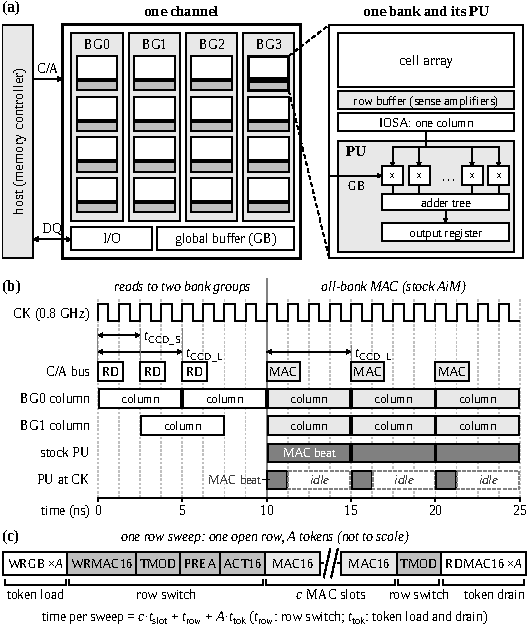
\includegraphics[width=\columnwidth]{figs/fig_dram_pim.pdf}
  \caption{AiM-style PIM: (a)~one channel and one bank with its PU; (b)~commands and MAC beats on the mobile platform; (c)~one row sweep.}
  \label{fig:dram_pim}
\end{figure}

% P:intro-prior-families
Prior PIM designs raise the ceiling in two families, and each family keeps every MAC paced by a DRAM command. The wider-PU
family spends multipliers: LP-Spec~\cite{lpspec} keeps one MAC step per column command and widens the step, feeding one
read to four 32-wide ALUs. The four ALUs carry four times the multipliers, and LP-Spec~\cite{lpspec} estimates that its
compute units and buffers take 16.92\,\% of an LPDDR5 die. The faster-PU family spends commands: P3-LLM~\cite{p3llm}
latches a weight and issues one command per token, so P3-LLM's MACs inherit the minimum command spacing \tccds, half the
column period: at most two tokens share a read.

% P:intro-timing-insight
Critically, DRAM timing parameters exist to meet DRAM access requirements by spacing the column commands that move data
out of the cell array~\cite{hbmpim}, not the MACs on a column already latched beside the bank. The column period
$t_\mathrm{col}$, the time one all-bank column command occupies the bank, sets how often a column arrives, and the PU
clock $f_\mathrm{PU}$ sets how often the PU computes, so one column can feed $D = t_\mathrm{col} \times f_\mathrm{PU}$
beats. An all-bank column lasts 5\,ns on LPDDR5-6400~\cite{lpspec} and 4\,ns on HBM2~\cite{hbmpim}, and a PU built in a
DRAM process runs at 1\,GHz in silicon~\cite{aimjssc}. A PU clocked at 0.8\,GHz on LPDDR5-6400 or at 1\,GHz on HBM2
fits $D = 4$ beats into each column period, of which a stock PU uses one.

% P:intro-code-proposal
To this end, this paper proposes CoDe (Command-Decoupled PIM). One column command reads a weight column once; the PU holds the
column and runs $D$ beats per column period over a tile of $V$ token vectors, at its own clock and the stock
multiplier count. We evaluate CoDe against each rival on that rival's own memory, workload and precision. On a mobile
platform (Snapdragon 8 Gen 3~\cite{sd8g3} SoC and NPU, PIM on x64 LPDDR5-6400, INT8), CoDe matches LP-Spec-style's
end-to-end decoding speed on 0.539$\times$ its logic area, so CoDe returns 1.87$\times$ LP-Spec-style's tokens per
second per logic mm$^2$. On an edge server with HBM2 at W4A8, CoDe decodes a batch of 8 1.68$\times$ faster than
P3-LLM-style, with 1.26$\times$ the throughput per logic mm$^2$ and 1.64$\times$ the system energy efficiency.

% P:intro-contributions
In summary, this paper makes the following contributions:
\begin{itemize}
  \item We identify that prior PIM ties MAC timing to DRAM command timing and derive the depth a column allows once
        MAC timing is separated from command timing: 4 beats on LPDDR5-6400 and HBM2 (Section~\ref{sec:bg:depth}).
  \item We propose CoDe, a PU and command extension that runs $D$ MAC beats per column command over a tile of tokens
        at the stock multiplier count (Section~\ref{sec:design}).
  \item We evaluate CoDe in two pairings on each rival's own ground: against LP-Spec-style on LPDDR5-6400 (INT8,
        speculative decoding) and against P3-LLM-style on HBM2 (W4A8, batched decoding) (Section~\ref{sec:eval}).
\end{itemize}

% float defined after page 1's right column has closed, so it renders at the top of page 2 (one float per column)
\begin{figure}[t]
  \centering
  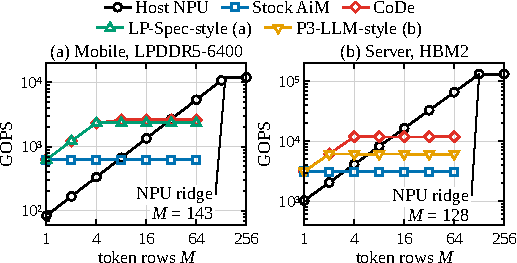
\includegraphics[width=\columnwidth]{figs/fig_roofline.pdf}
  \caption{Skinny-GEMM throughput against the number of token rows $M$: (a)~mobile platform; (b)~edge server.}
  \label{fig:roofline}
\end{figure}
